
La interacción entre los distintos servicios que se desarrollan en este proyecto se realizarán mediante una API. Entre los dos paradígmas más utilizados a la hora de crear APIs se encuentran RPC y REST. Se va a escoger el estandar RPC por responder a los requisistos a los que nos enfrentamos.

\textbf{GRPC}

Según el paper original que describe el paradígma RPC ¨Remote procedure calls (RPC) appear to be a useful paradig m for providing communication across a
network between programs written in a high-level language.¨ \cite{Birrell198439}

RPC permite ejecutar una llamada a un servicio en un servidor remoto mediante formularios predefinidos, obteniendo respuestas con el mismo formato. El estilo del servidor que realiza la llamada, no se tiene en cuenta por diseño.

Google Remote Procedure Call \cite{grpc} - es un subtipo del diseño RPC. gRPC es una arquitectura global de alto rendimiento y de código abierto RPC que garantiza la flexibilidad y la velocidad de la arquitectura de microservicios. Las llamadas a funciones se utilizan gRPC para garantizar la interacción con el cliente en los microservicios creados con varios lenguajes de codificación.

Esta técnica implementa las peticiones de la API en RPC utilizando el estándar HTTP 2.0, pero ni el servidor ni el programador de la API tienen conocimiento de HTTP. Como resultado, la complicación disminuye porque no hay que preocuparse por cómo se traducen los principios de RPC a HTTP.

La llamada a procedimientos remotos de Google pretende acelerar la transferencia de datos entre microservicios. Para permitir la devolución y la llamada remotas, se basa en una estrategia que identifica un servicio, establece las metodologías y especifica las variables pertinentes.

Además, utiliza un IDL -lenguaje de descripción de interfaces- para especificar el paradigma de la API RPC, lo que simplifica la identificación de las funciones remotas. El IDL emplea por defecto Protocol Buffers para definir la interfaz del servicio y el formato de los mensajes de carga útil.

\textbf{REST}

REST - Representational State Transfer - es un paradigma cliente-servidor se comunican a través de mensajes codificados en formato JSON o XML o compatibles.

En su disertación original del año 2000, Roy T. Fielding define REST como un "It means that a server will respond with the representation of a resource (today, it will most often be an HTML, XML or JSON document) and that resource will contain hypermedia links that can be followed to make the state of the system change. Any such request will in turn receive the representation of a resource, and so on." \cite{FieldingRoyThomas2000Asat}

Los principios que lo describen son:

\begin{itemize}
    \item Arquitectura cliente-servidor. Hace hincapié en la separación de responsabilidades.
    \item Ausencia de estado. El estado se guarda y mantiene en el cliente y no en el servidor
    \item Habilitación y uso de la caché. Todas las solicitudes deben declarar si son o no cacheables,
    \item Interfaz unifome
    \item Sistema por capas. Tiene relación con la separación de responsabilidades
\end{itemize}

Cada componente que combina el sistema de microservicios puede mostrarse al usuario o al cliente como un recurso cuando la API REST se hace accesible públicamente. Este recurso puede consultarse mediante los comandos HTTP GET, POST, PUT y DELETE .

En una API RESTful, el usuario envía una consulta a una URL - Localizador Uniforme de Recursos, que provoca una respuesta con una carga útil en JSON, XML o cualquier formato de datos compatible. Esta carga útil representa el recurso que desea el usuario. Las peticiones comunes de los clientes incluyen

\begin{itemize}
    \item Un método HTTP que especifica lo que debe procesarse en el recurso
    \item La ruta del recurso
    \item La cabecera que contiene datos sobre la consulta
    \item Una carga útil de mensaje específica del cliente
\end{itemize}

El servidor de la API envía una cabecera de tipo de contenido que identifica el formato de entrega del mensaje empleado en el cuerpo de la respuesta junto con la carga útil de datos que entrega al usuario que realiza la consulta. También se incluye en el cuerpo de la respuesta un código de respuesta que informa al usuario del estado del resultado de la llamada a la API.

\textbf{HTTP 1.1 frente a HTTP 2}

El protocolo HTTP/2 para transmitir mensajes permite flujos multiplexados y una comunicación bidireccional. gRPC admite varios tipos de interacciones, incluyendo interacciones unarias, streaming de servidor, streaming de cliente y streaming bidireccional. En contraste, REST utiliza el modelo de petición-respuesta de HTTP 1.1, lo que puede causar problemas de latencia y no aprovechar completamente las ventajas de HTTP/2. En general, gRPC puede proporcionar una transmisión de datos más rápida y eficiente y una comunicación más flexible y bidireccional en comparación con REST. HTTP 1.1, que permite REST, utiliza un método de handshaking TCP para cada consulta. REST Por ello, las APIs suelen tener problemas de latencia, ya que el handshake lleva tiempo.

\textbf{La estructura de datos de la carga útil}

Si nos fijamos en la estructura de datos de la carga útil, utilizada en el intercambio que se produce en la comunicación, gRPC utiliza Protocol Buffers para serializar y deserializar datos, lo que permite una transmisión más rápida y eficiente de información. Este método es más ligero, ya que los mensajes son una estructura más comprimida. Están en formato binario, lo que hace que el procesamiento sea menos intensivo en CPU. En el intercambio de datos, serializa y deserializa la información de forma automática.

Por otro lado, en REST, se utiliza principalmente JSON o XML para enviar y recibir información. La facilidad de lectura humana de JSON es una ventaja de REST, pero no es tan rápido o ligero cuando se trata de la transferencia de datos. Esto se debe al requerimiento de que JSON debe ser serializado y traducido a los lenguajes de programación utilizados en ambos extremos, el servidor y el cliente. Este paso adicional en el proceso de transmisión de datos puede afectar la eficiencia y aumentar la probabilidad de errores.


\textbf{Compatibilidad con los navegadores}\label{GRPCcompatibilidadConNavegadores}

Dado que la mayor parte de la interacción de la API web se produce en línea, la compatibilidad con el navegador es una consideración clave en el debate entre gRPC vs. REST. La compatibilidad con los navegadores es probablemente una de las principales ventajas de las APIs REST frente a gRPC. Todos los navegadores ofrecen la capacidad completa de la API REST y la compatibilidad con el navegador. Sin embargo, para gRPC los navegadores sigue siendo relativamente restringida.

Para la comunicación entre HTTP 1.1 y HTTP 2 que necesita la interacción entre la web y gRPC se hace necesario establecer una capa proxy; lo cual presenta un elemento más de complejidad y mantenimiento, es por lo tanto un inconveniente en el uso de gRPC.

\textbf{Generación de código}

Para gRPC existe un compilador llamado protoc que carga los archivos .proto y genera código nativo para comunicarse con los servicios remotos que admite múltiples lenguajes de programación. En REST los ingenieros deben emplear herramientas de terceros, como Postman, para la generación de código para las consultas de la API.

La generación de código es especialmente ventajosa para los microservicios que combinan numerosos servicios creados en múltiples plataformas y lenguajes, facilitando la construcción del kit de desarrollo de software (SDK) para cada lenguaje y actualizándose de forma sencilla cuando se enfrenta a cambios.

\textbf{Justificación de uso de gRPC}

Aunque actualmente la mayoría de las herramientas de terceros no ofrecen una funcionalidad integrada para gRPC, es una tecnología adecuada para la interacción entre sistemas internos, como microservicios. Además, gRPC permite la interoperabilidad entre distintos lenguajes de programación, lo cual es otro de sus puntos fuertes. Esto se logra mediante el sistema generador de código, que se produce utilizando los archivos proto como interfaz de comunicación, lo que brinda una herramienta útil para aquellos que desean agregar funcionalidades mediante otro lenguaje y comunicarse fácilmente con el sistema ya existente. Todo lo que se necesita hacer es compilar los archivos proto en el lenguaje destino.

Otro beneficio del uso de gRPC es la transmisión de información en tiempo real mediante buffers de comunicación. En nuestro caso, el control en tiempo real de dispositivos mediante sistemas PID hace que esta característica sea esencial. gRPC permite establecer conexiones tanto de streaming por parte del cliente como del servidor, lo que nos permite establecer canales de comunicación versátiles según la situación a la que nos enfrentemos. Además, para la monitorización de los dispositivos controlados, necesitamos una optimización en el uso del ancho de banda. Aquí es donde gRPC sobresale, ya que proporciona una comunicación ligera, mayor eficiencia y rapidez.


Como resumén final hacemos referencia a a figura \ref{fig:gRPC vs REST} que resume la comparación entre los dos sistemas

\begin{figure}[H]
    \centering
    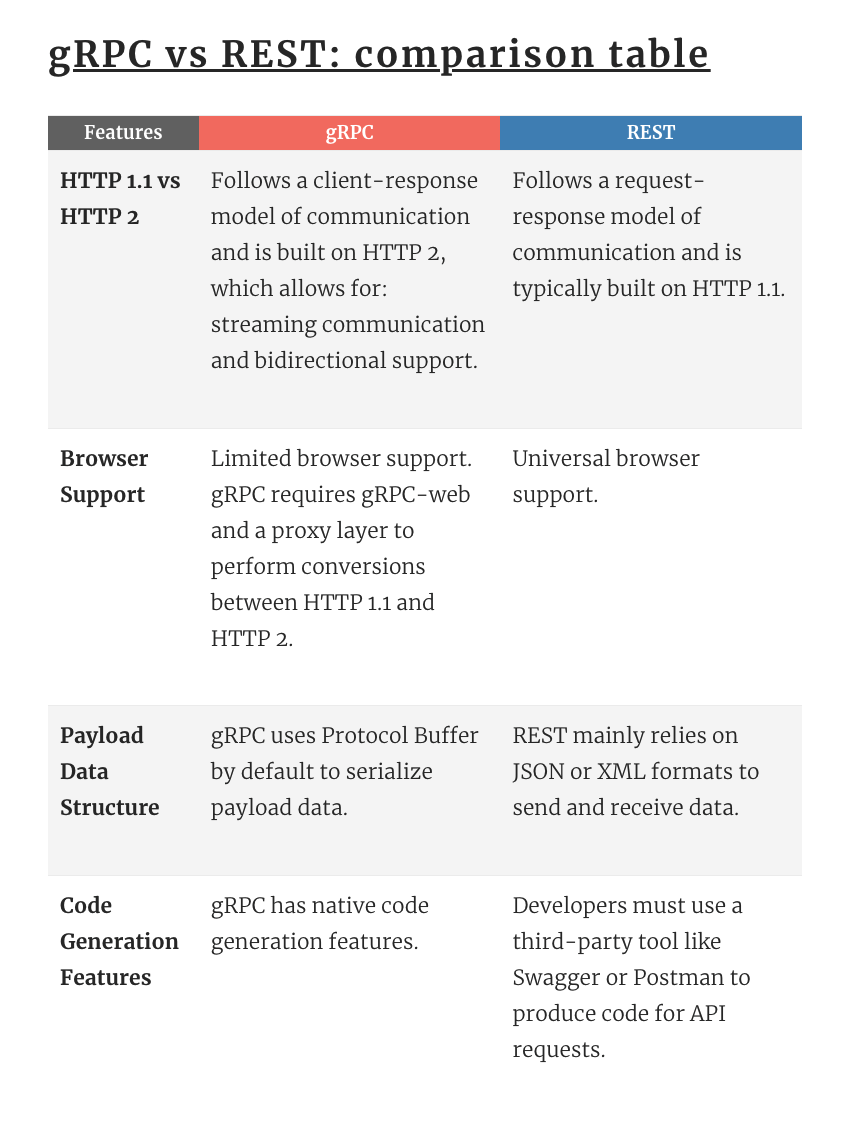
\includegraphics[height=0.3\textheight]{./part/Proyecto_ejecutivo/memoria_constructiva/rpc/img/rpcComparison}
    \caption{gRPC vs REST.\cite{berga_santos_2023}}\label{fig:gRPC vs REST}
\end{figure}